\documentclass[aspectratio=169, table]{beamer}

\usepackage{colortbl}
\usepackage{xcolor}
\usepackage{listings}
\usepackage{xcolor}
\usepackage{pgfplots}
\usepgfplotslibrary{polar}
\usepackage{tikz}
\usetikzlibrary{shapes.geometric, 
	positioning, shapes, shapes.multipart, backgrounds, arrows.meta, calc, fit, trees}

\usetheme{Pradita}



\lstdefinelanguage{bash} {
	keywords={},
	basicstyle=\ttfamily\scriptsize,
	keywordstyle=\color{blue}\bfseries,
	ndkeywords={iex},
	ndkeywordstyle=\color{purple}\bfseries,
	sensitive=true,
	commentstyle=\color{gray},
	stringstyle=\color{red},
	numbers=left,
	numberstyle=\tiny\color{gray},
	breaklines=true,
	frame=lines,
	backgroundcolor=\color{lightgray!10},
	tabsize=2,
	comment=[l]{\#},
	morecomment=[s]{/*}{*/},
	commentstyle=\color{gray}\ttfamily,
	stringstyle=\color{purple}\ttfamily,
	showstringspaces=false,
	captionpos=b
}

% Define Python language style for listings
\lstdefinestyle{PythonStyle}{
    language=Python,
    basicstyle=\ttfamily\footnotesize,
    keywordstyle=\color{blue}\bfseries,
    commentstyle=\color{gray}\itshape,
    stringstyle=\color{red},
    showstringspaces=false,
    breaklines=true,
    frame=lines,
    numbers=left,
    numberstyle=\tiny\color{gray},
    backgroundcolor=\color{lightgray!10},
    tabsize=4,
    captionpos=b
}

\lstdefinelanguage{terraform} {
	keywords={variable, bool, type, number, string, default, locals, resource, dynamic, 
				module, content, output},
	basicstyle=\ttfamily\scriptsize,
	keywordstyle=\color{blue}\bfseries,
	ndkeywords={iex},
	ndkeywordstyle=\color{purple}\bfseries,
	sensitive=true,
	commentstyle=\color{gray},
	stringstyle=\color{red},
	numbers=left,
	numberstyle=\tiny\color{gray},
	breaklines=true,
	frame=lines,
	backgroundcolor=\color{lightgray!10},
	tabsize=2,
	comment=[l]{\#},
	morecomment=[s]{/*}{*/},
	string=[s]{'}{'},
	morestring=[s]{"}{"},
	commentstyle=\color{gray}\ttfamily,
	stringstyle=\color{purple}\ttfamily,
	showstringspaces=false
}


\subtitle{IT30213 - Advanced Software Engineering \& DevOps}
\title{\Huge Software Infrastructure\\\vspace{8pt}	
	Orchestration\vspace{5pt}}
%\date[Serial]{Penggunaan Large Language Model untuk Pengajaran}
\author{\textbf{Alfa Yohannis}}
\begin{document}
	
	\frame{\titlepage}
	

	\begin{frame}[fragile]
		\frametitle{Contents}
		\vspace{20pt}
		\begin{columns}[t]
			\column{0.5\textwidth}
			\tableofcontents[sections={1-5}]
			
			\column{0.5\textwidth}
			\tableofcontents[sections={6-20}]
		\end{columns}
	\end{frame}
	
	\begin{frame}{\hfill}
		\centering
		\Huge{\textbf{How to manage software infrastructure at runtime?}}
	\end{frame}
	
\section{Pendahuluan}
\begin{frame}{\hfill}
	\centering
	\Huge{\textbf{Pendahuluan}}
\end{frame}

\begin{frame}{Pendahuluan}
\vspace{20pt}
Perangkat lunak modern tidak lagi berjalan sebagai satu program pada satu mesin.
Sistem dibangun sebagai \textbf{microservices} dalam container yang saling berkomunikasi melalui jaringan. Pendekatan ini meningkatkan fleksibilitas dan skalabilitas, namun menambah \textbf{kompleksitas operasional}.

\vspace{6pt}
\textbf{Tantangan utama:}
\begin{itemize}
    \item Menjaga aplikasi tetap berjalan saat terjadi kegagalan.
    \item Menambah/mengurangi instance sesuai beban.
    \item Melakukan pembaruan tanpa downtime.
    \item Mengelola komunikasi layanan tanpa IP manual.
\end{itemize}

\vspace{10pt}
Pengelolaan manual tidak lagi memadai.
Diperlukan sistem orkestrasi container yang otomatis, adaptif, dan terkontrol.
\end{frame}

\section{Definisi Kubernetes}
\begin{frame}{\hfill}
	\centering
	\Huge{\textbf{Definisi Kubernetes}}
\end{frame}

\begin{frame}{Definisi Kubernetes}
\vspace{20pt}
\textbf{Kubernetes} adalah platform orkestrasi container \textit{open-source} 
untuk mengelola deployment, scaling, dan operasi aplikasi berbasis container secara otomatis.

\vspace{6pt}
Secara konseptual, Kubernetes bersifat \textbf{deklaratif}. 
Pengguna mendefinisikan \textit{desired state}, bukan langkah prosedural.

\vspace{6pt}
\textbf{Contoh:}
\begin{itemize}
    \item Aplikasi API harus memiliki \textbf{3 replica}.
    \item Jika 1 Pod gagal $\rightarrow$ dibuat ulang otomatis.
    \item Jika beban naik $\rightarrow$ replica ditambah.
    \item Jika beban turun $\rightarrow$ replica dikurangi.
\end{itemize}

\vspace{6pt}
Dengan mekanisme ini, Kubernetes bertindak sebagai 
\textbf{sistem kontrol terdistribusi} yang menjaga stabilitas, 
ketersediaan, dan elastisitas aplikasi secara kontinu.
\end{frame}


\section{Arsitektur dan Cara Kerja Kubernetes}
\begin{frame}{\hfill}
	\centering
	\Huge{\textbf{Arsitektur dan Cara Kerja Kubernetes}}
\end{frame}

\begin{frame}{\LARGE{Arsitektur Kubernetes: Control Plane vs Worker Node}}
\vspace{15pt}
\centering
\scalebox{0.45}{
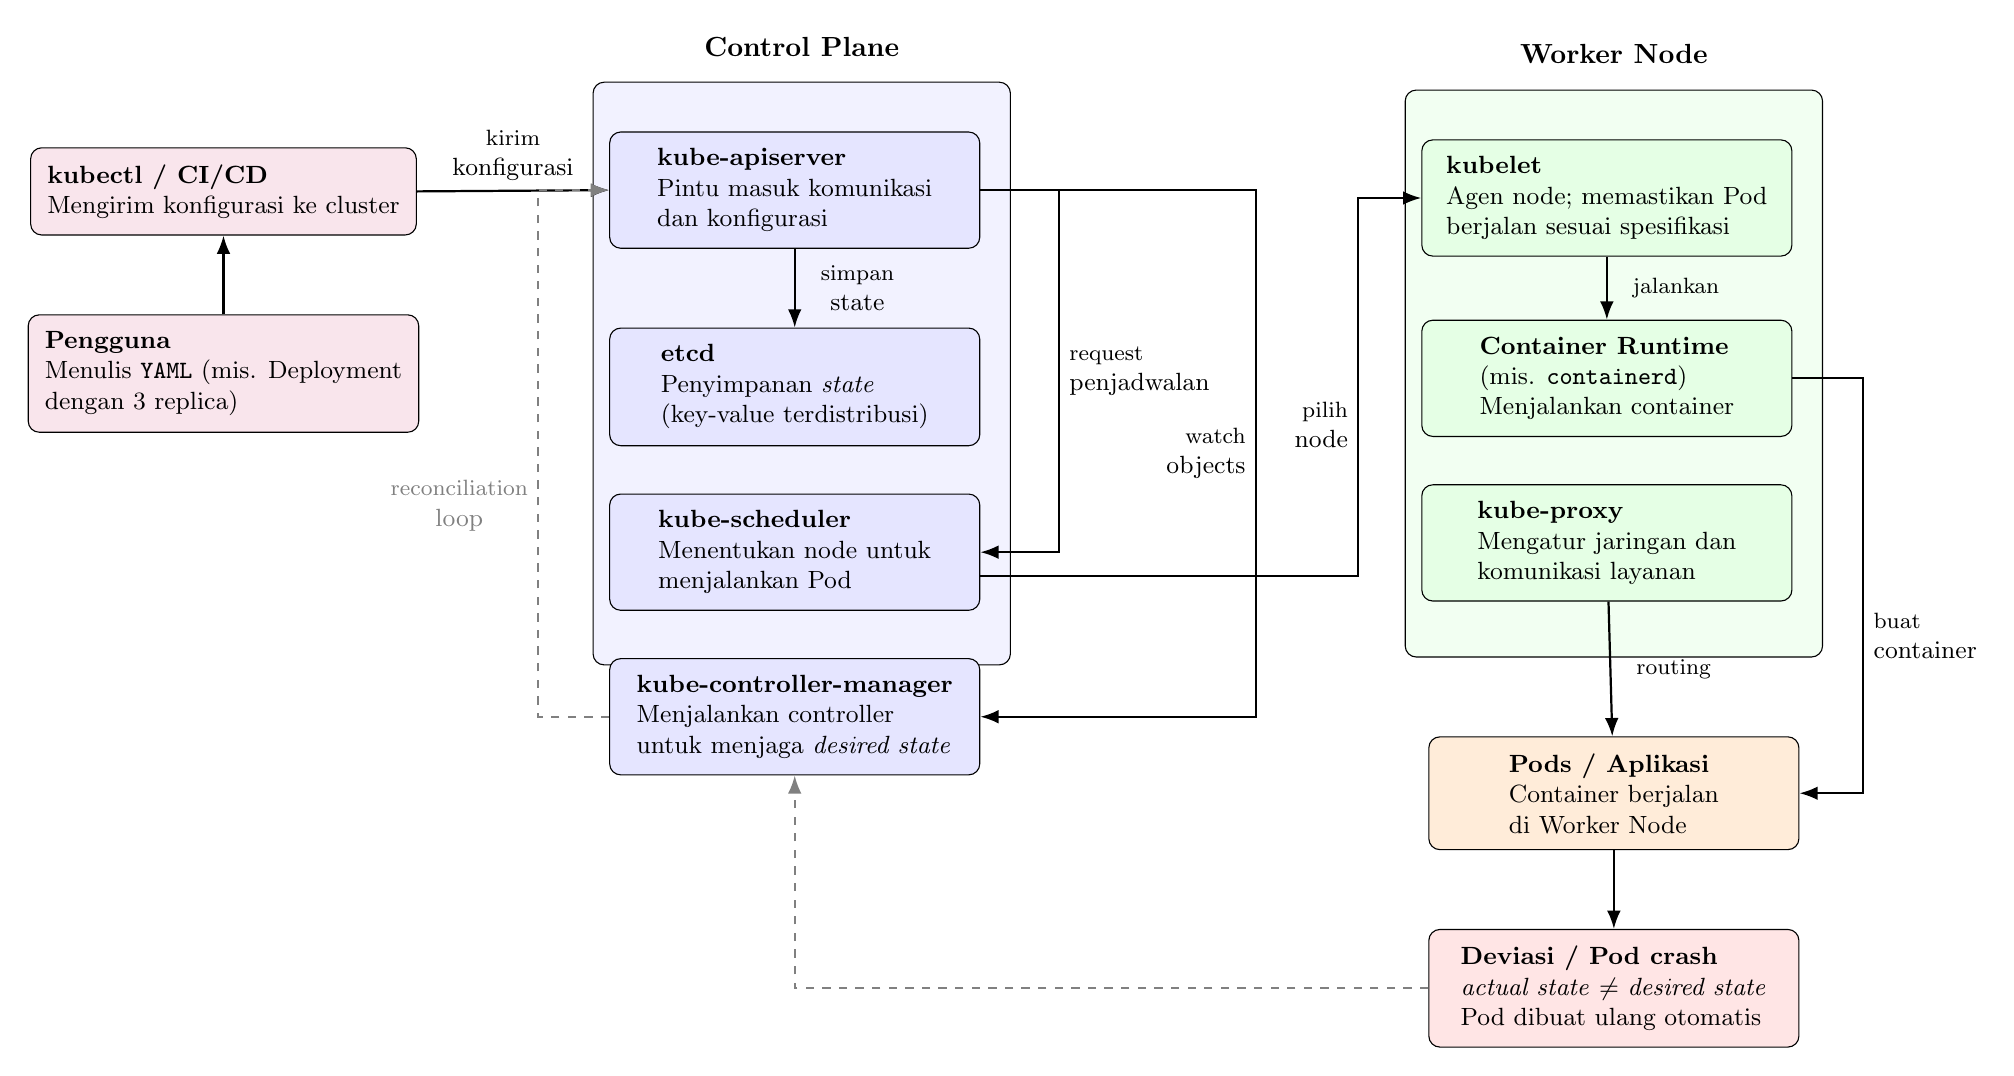
\begin{tikzpicture}[
  font=\small,
  box/.style={draw, rounded corners, align=left, inner sep=6pt, minimum width=4.2cm, fill=white},
  bigbox/.style={draw, rounded corners, align=left, inner sep=8pt, minimum width=5.3cm},
  title/.style={font=\bfseries},
  arrow/.style={-Latex, thick}
]

% ===== User + YAML =====

\node[box, fill=purple!10] (kubectl) {\textbf{kubectl / CI/CD}\\
Mengirim konfigurasi ke cluster};

\node[box, fill=purple!10, below=10mm of kubectl] (user) {\textbf{Pengguna}\\
Menulis \texttt{YAML} (mis. Deployment\\dengan 3 replica)};

\draw[arrow] (user) -- (kubectl);

% ===== Control Plane =====
\node[bigbox, fill=blue!5, right=22mm of user, minimum height=7.4cm, inner sep=12pt] (cp) {};
\node[font=\bfseries, above=2mm of cp] {Control Plane};

\node[box, fill=blue!10, anchor=north west, minimum width=4.7cm] (apiserver)
  at ([xshift=6pt,yshift=-18pt]cp.north west)
{\textbf{kube-apiserver}\\
Pintu masuk komunikasi\\dan konfigurasi};

\node[box, fill=blue!10, below=10mm of apiserver, minimum width=4.7cm] (etcd)
{\textbf{etcd}\\
Penyimpanan \textit{state}\\(key-value terdistribusi)};

\node[box, fill=blue!10, below=6mm of etcd, minimum width=4.7cm] (scheduler)
{\textbf{kube-scheduler}\\
Menentukan node untuk\\menjalankan Pod};

\node[box, fill=blue!10, below=6mm of scheduler, minimum width=4.7cm] (controller)
{\textbf{kube-controller-manager}\\
Menjalankan controller\\untuk menjaga \textit{desired state}};

% ===== Worker Node =====
\node[bigbox, fill=green!5, right=50mm of cp, minimum height=7.2cm, inner sep=12pt] (wn) {};
\node[font=\bfseries, above=2mm of wn] {Worker Node};

\node[box, fill=green!10, anchor=north west, minimum width=4.7cm] (kubelet)
  at ([xshift=6pt,yshift=-18pt]wn.north west)
{\textbf{kubelet}\\
Agen node; memastikan Pod\\berjalan sesuai spesifikasi};

\node[box, fill=green!10, below=8mm of kubelet, minimum width=4.7cm] (runtime)
{\textbf{Container Runtime}\\
(mis. \texttt{containerd})\\Menjalankan container};

\node[box, fill=green!10, below=6mm of runtime, minimum width=4.7cm] (proxy)
{\textbf{kube-proxy}\\
Mengatur jaringan dan\\komunikasi layanan};

\node[box, fill=orange!15, below=10mm of wn, minimum width=4.7cm] (pods)
{\textbf{Pods / Aplikasi}\\
Container berjalan\\di Worker Node};

% ===== Main flow =====
\draw[arrow] (kubectl.east) -- node[above, align=center]{\footnotesize kirim\\konfigurasi} (apiserver.west);

\draw[arrow]
  (apiserver) -- 
  node[right, xshift=2mm, align=center]
  {\footnotesize simpan\\state}
  (etcd);

\draw[arrow] (apiserver.east) -- ++(10mm,0) |- node[pos=0.25, right, align=left]{\footnotesize request\\penjadwalan} (scheduler.east);

\draw[arrow] (apiserver.east) -- ++(35mm,0) |- node[pos=0.25, left, align=right]{\footnotesize watch\\objects} (controller.east);

\draw[arrow, dashed, gray]
  (controller.west) -- ++(-9mm,0) |-
  node[pos=0.35, left, yshift=-20mm, align=center]
  {\footnotesize reconciliation\\loop}
  (apiserver.west);

\draw[arrow] 
  ([yshift=-3mm]scheduler.east) -- ++(48mm,0) 
  |- node[pos=0.2, left, align=right]
     {\footnotesize pilih\\node} 
  (kubelet.west);

\draw[arrow] (kubelet) -- node[right, xshift=2mm, align=center]{\footnotesize jalankan} (runtime);

\draw[arrow] (runtime.east) --  ++(9mm,0) |- node[right, yshift=20mm, align=left]{\footnotesize buat\\container} (pods);

\draw[arrow] (proxy) -- node[right, xshift=2mm, align=center]{\footnotesize routing} (pods);

% ===== Self-healing note =====
\node[box, fill=red!10, below=10mm of pods, minimum width=4.7cm] (crash)
{\textbf{Deviasi / Pod crash}\\
\textit{actual state} $\neq$ \textit{desired state}\\
Pod dibuat ulang otomatis};

\draw[arrow] (pods) -- (crash);
\draw[arrow, dashed, gray] (crash.west)  -- ++(-10mm,0) -| (controller.south);

\end{tikzpicture}
}

\vspace{2pt}
{\small\textit{Desired state} disimpan di \textbf{etcd}; controller menjalankan \textbf{reconciliation loop} untuk \textbf{self-healing}.}
\end{frame}

\begin{frame}{Arsitektur dan Komponen Kubernetes}
\vspace{10pt}
\textbf{Kubernetes} terbagi menjadi dua bagian utama:

\vspace{6pt}
\textbf{1. Control Plane (Pusat Kendali)}
\begin{itemize}
    \item \textbf{kube-apiserver} $\rightarrow$ pintu masuk seluruh komunikasi cluster.
    \item \textbf{etcd} $\rightarrow$ database key-value terdistribusi penyimpan \textit{state}.
    \item \textbf{kube-scheduler} $\rightarrow$ menentukan node untuk menjalankan Pod.
    \item \textbf{kube-controller-manager} $\rightarrow$ menjalankan controller menjaga \textit{desired state}.
\end{itemize}

\vspace{6pt}
\textbf{2. Worker Node (Eksekusi Aplikasi)}
\begin{itemize}
    \item \textbf{kubelet} $\rightarrow$ memastikan Pod berjalan sesuai spesifikasi.
    \item \textbf{Container Runtime} (mis. \texttt{containerd}) $\rightarrow$ menjalankan container.
    \item \textbf{kube-proxy} $\rightarrow$ mengatur komunikasi jaringan layanan.
\end{itemize}

\vspace{4pt}
\small
Pemisahan ini membedakan kendali sistem dan eksekusi aplikasi.
\end{frame}

\begin{frame}{Bagaimana Kubernetes Bekerja}
\vspace{10pt}
Kubernetes bekerja dengan prinsip \textbf{reconciliation loop}:
membandingkan \textit{actual state} dengan \textit{desired state} secara kontinu.

\vspace{6pt}
\textbf{Alur Kerja:}
\begin{enumerate}
    \item Pengguna menulis konfigurasi YAML (mis. Deployment 3 replica).
    \item Konfigurasi dikirim ke \textbf{kube-apiserver}.
    \item State disimpan di \textbf{etcd}.
    \item Controller memonitor kesesuaian kondisi aktual.
    \item Jika terjadi deviasi (mis. Pod crash), sistem membuat ulang otomatis.
\end{enumerate}

\vspace{6pt}
\textbf{Karakteristik:}
\begin{itemize}
    \item Deklaratif, Self-healing, Adaptif terhadap perubahan beban, Beroperasi kontinu, bukan sekali eksekusi.
\end{itemize}
\end{frame}

\section{Struktur Direktori}
\begin{frame}{\hfill}
	\centering
	\Huge{\textbf{Struktur Direktori}}
\end{frame}

\begin{frame}[fragile]{Struktur Proyek Kubernetes (Base \& Overlays)}
\vspace{10pt}
\begin{columns}[T]

% ===== LEFT COLUMN =====
\column{0.52\textwidth}
\textbf{Base (Reusable Definition)}
\begin{lstlisting}[language=bash]
kubernetes/
|-- base
|   |-- namespace.yaml
|   |-- configmap-app.yaml
|   |-- secret-app.yaml
|   |-- deploy-api.yaml
|   |-- deploy-web.yaml
|   |-- deploy-worker.yaml
|   |-- deploy-redis.yaml
|   |-- statefulset-minio.yaml
|   |-- svc-api.yaml
|   |-- svc-web.yaml
|   |-- svc-redis.yaml
|   |-- svc-minio.yaml
|   |-- hpa-worker.yaml
|   |-- ingress.yaml
|   `-- kustomization.yaml
\end{lstlisting}

% ===== RIGHT COLUMN =====
\column{0.48\textwidth}
\textbf{Overlays (Environment-Specific)}
\begin{lstlisting}[language=bash]
`-- overlays
    |-- dev
    |   |-- patch-env.yaml
    |   |-- patch-images.yaml
    |   `-- kustomization.yaml
    |-- staging
    |   |-- patch-configmap.yaml
    |   |-- patch-replicas.yaml
    |   `-- kustomization.yaml
    `-- prod
        |-- patch-configmap.yaml
        |-- patch-replicas.yaml
        |-- pdb-api.yaml
        |-- pdb-web.yaml
        `-- kustomization.yaml
\end{lstlisting}
\scriptsize
Prinsip: \textbf{base sama} $\rightarrow$ \textbf{patch berbeda} $\rightarrow$ multi-environment tanpa duplikasi YAML.
\end{columns}

\end{frame}



\begin{frame}{Struktur Direktori (Base \& Overlays)}
\vspace{10pt}
\begin{columns}[T]

% ===== LEFT COLUMN =====
\column{0.5\textwidth}
\textbf{Direktori \texttt{base}}
\begin{itemize}
    \item \textbf{Environment-agnostic} (model dasar).
    \item Namespace → isolasi resource.
    \item ConfigMap \& Secret → pisahkan konfigurasi dan kredensial.
    \item Deployment stateless: API, Web, Worker, Redis.
    \item StatefulSet + PVC → MinIO (durabilitas data).
    \item Service + Ingress → abstraksi jaringan.
    \item HPA + Job → autoscaling dan bootstrap otomatis.
\end{itemize}

% ===== RIGHT COLUMN =====
\column{0.5\textwidth}
\textbf{Direktori \texttt{overlays}}
\begin{itemize}
    \item Mewarisi \texttt{../../base}.
    \item Patch environment variable (\texttt{patch-env.yaml}).
    \item Patch image tag (promosi CI/CD).
    \item Patch replica (kapasitas per env).
    \item Domain berbeda: dev, staging, prod.
    \item Prod → tambah PodDisruptionBudget (high availability).
\end{itemize}

\vspace{6pt}
\small
Prinsip: \textbf{base = model infrastruktur}, 
overlay = variasi kontekstual tanpa duplikasi YAML.
\end{columns}
\end{frame}

\section{Demo}
\begin{frame}{\hfill}
	\centering
	\Huge{\textbf{Demo}}
\end{frame}


\begin{frame}[fragile]{(1) Instalasi \& Inisialisasi Minikube}
\vspace{10pt}
\begin{columns}[T]
\column{0.52\textwidth}
\textbf{Reset cluster (jika pernah ada)}
\begin{lstlisting}[language=bash]
minikube stop
minikube delete
\end{lstlisting}

\textbf{Start Minikube (simulasi prod)}
\begin{lstlisting}[language=bash]
minikube start --cpus=4 --memory=8192
\end{lstlisting}

\column{0.48\textwidth}
\textbf{Aktifkan addon wajib}
\begin{lstlisting}[language=bash]
minikube addons enable ingress
minikube addons enable metrics-server
\end{lstlisting}

\begin{itemize}
  \item \textbf{ingress}: routing HTTP eksternal.
  \item \textbf{metrics-server}: metrik CPU untuk HPA.
  \item Pastikan Docker daemon sedang berjalan.
\end{itemize}
\end{columns}
\end{frame}

\begin{frame}[fragile]{(2) Memuat Image Lokal ke Minikube}
\vspace{10pt}
\begin{columns}[T]
\column{0.62\textwidth}
\textbf{Load image (production)}
\begin{lstlisting}[language=bash]
minikube image load session05-api:production
minikube image load session05-web:production
minikube image load session05-worker:production
minikube image load redis:7-alpine
minikube image load minio/minio:RELEASE.2025-09-07T16-13-09Z
\end{lstlisting}

\column{0.38\textwidth}
\textbf{Verifikasi}
\begin{lstlisting}[language=bash]
minikube image ls
\end{lstlisting}

\begin{itemize}
  \item Wajib jika cluster tidak pull dari registry.
  \item Pastikan tag image sesuai manifest/patch.
\end{itemize}
\end{columns}
\end{frame}

\begin{frame}[fragile]{(3) Deploy Overlay Production \& Uji Endpoint}
\vspace{10pt}
\begin{columns}[T]
\column{0.55\textwidth}
\textbf{Deploy resource production}
\begin{lstlisting}[language=bash]
kubectl apply -k ./overlays/prod
\end{lstlisting}

\textbf{Cek komponen}
\begin{lstlisting}[language=bash]
kubectl get all -n tts
kubectl get ingress -n tts -o wide
\end{lstlisting}

\column{0.45\textwidth}
\textbf{Aktifkan akses eksternal}
\begin{lstlisting}[language=bash]
minikube tunnel
minikube ip
\end{lstlisting}

\textbf{Uji health endpoint}
\begin{lstlisting}[language=bash]
curl -i -H "Host: tts.local" \
  http://<MINIKUBE_IP>/api/healthz
\end{lstlisting}

\begin{itemize}
  \item Ekspektasi: HTTP 200.
\end{itemize}
\end{columns}
\end{frame}

\begin{frame}[fragile]{(4) Rolling Update (Tanpa Downtime Total)}
\vspace{10pt}
\begin{columns}[T]
\column{0.62\textwidth}
\textbf{Update image secara rolling}
\begin{lstlisting}[language=bash]
kubectl set image -n tts deploy/api \
  api=session05-api:production
kubectl rollout status -n tts deploy/api
\end{lstlisting}

\textbf{Amati pergantian pod}
\begin{lstlisting}[language=bash]
kubectl get pods -n tts -w
\end{lstlisting}

\column{0.38\textwidth}
\begin{itemize}
  \item Pod diganti bertahap.
  \item Service tetap melayani request.
  \item Cocok untuk perubahan versi di production.
\end{itemize}
\end{columns}
\end{frame}


\begin{frame}[fragile]{(5) Self-Healing: Uji Reconciliation Loop}
\vspace{10pt}
\begin{columns}[T]
\column{0.58\textwidth}
\textbf{Hapus satu pod manual}
\begin{lstlisting}[language=bash]
kubectl delete pod -n tts <nama-pod>
kubectl get pods -n tts -w
\end{lstlisting}

\column{0.42\textwidth}
\begin{itemize}
  \item \textit{desired state} tetap sama.
  \item Controller membuat pod baru otomatis.
  \item Inilah mekanisme \textbf{reconciliation loop}.
\end{itemize}
\end{columns}
\end{frame}


\begin{frame}[fragile]{(6) HPA: Scale Up/Down Berbasis Beban}
\vspace{10pt}
\begin{columns}[T]
\column{0.54\textwidth}
\textbf{Pantau HPA}
\begin{lstlisting}[language=bash]
kubectl get hpa -n tts
watch -n 1 kubectl get hpa -n tts
\end{lstlisting}

\textbf{Generate beban}
\begin{lstlisting}[language=bash]
python ../../app/client/load_client.py \
  --base-url http://tts.local \
  --concurrency 20 --jobs 20 --check-mp3
\end{lstlisting}

\column{0.46\textwidth}
\textbf{Alternatif benchmarking}
\begin{lstlisting}[language=bash]
hey -n 2000 -c 50 \
  http://tts.local/api/healthz
\end{lstlisting}

\begin{itemize}
  \item Amati worker bertambah saat CPU naik.
  \item Turun kembali saat beban menurun.
\end{itemize}
\end{columns}
\end{frame}

\begin{frame}[fragile]{(7) Validasi Konfigurasi Production \& Image}
\vspace{10pt}
\begin{columns}[T]
\column{0.58\textwidth}
\textbf{Pastikan env terpasang}
\begin{lstlisting}[language=bash]
kubectl exec -n tts deploy/api -- \
  printenv | egrep 'ENV|MP3_BUCKET'
kubectl get configmap -n tts tts-config -o yaml
\end{lstlisting}

\column{0.42\textwidth}
\textbf{Verifikasi image runtime}
\begin{lstlisting}[language=bash]
kubectl get deploy -n tts api \
  -o jsonpath='{.spec.template.spec.containers[0].image}'; echo
\end{lstlisting}

\begin{itemize}
  \item Hindari mismatch antara overlay dan cluster.
\end{itemize}
\end{columns}
\end{frame}

\begin{frame}[fragile]{\LARGE{(8) Stateful Resilience: MinIO + Persistent Volume}}
\vspace{10pt}
\begin{columns}[T]
\column{0.52\textwidth}
\textbf{Uji restart pod MinIO}
\begin{lstlisting}[language=bash]
kubectl delete pod -n tts minio-0
kubectl get pods -n tts -w
\end{lstlisting}

\column{0.48\textwidth}
\begin{itemize}
  \item Pod dibuat ulang otomatis.
  \item Data tetap tersedia karena \textbf{PVC/PV}.
  \item StatefulSet menjaga identitas pod stabil.
\end{itemize}
\end{columns}
\end{frame}

\section{Kelebihan Kubernetes}
\begin{frame}{\hfill}
	\centering
	\Huge{\textbf{Kelebihan Kubernetes}}
\end{frame}

\begin{frame}{Kelebihan Kubernetes terhadap Terraform}
\vspace{10pt}
\begin{columns}[T]

\column{0.5\textwidth}
\textbf{Mental Model}
\begin{itemize}
    \item \textbf{Terraform} $\rightarrow$ Lifecycle Infrastruktur
    \item \textbf{Kubernetes} $\rightarrow$ Lifecycle Aplikasi
\end{itemize}

\vspace{6pt}
\textbf{Terraform}
\begin{itemize}
    \item Provisioning VM, network, storage
    \item \texttt{apply} sekali, selesai
\end{itemize}

\column{0.5\textwidth}
\textbf{Kubernetes}
\begin{itemize}
    \item Reconciliation loop
    \item Self-healing
    \item Auto scaling (naik \& turun)
    \item Rolling update
    \item Runtime orchestration
    \item Service discovery
\end{itemize}

\end{columns}
\end{frame}

% ============================================================
\begin{frame}[fragile]{Demo 1: Self-Healing}
\vspace{10pt}
\begin{columns}[T]

\column{0.52\textwidth}
\begin{lstlisting}[language=bash]
kubectl get pods -n tts
kubectl delete pod -n tts <nama-pod-api>
kubectl get pods -n tts -w
\end{lstlisting}

\column{0.48\textwidth}
\textbf{Observasi}
\begin{itemize}
    \item Pod dibuat ulang otomatis
    \item Desired state tetap terjaga
\end{itemize}

\textbf{Teaching Line}

Terraform tidak melakukan apa-apa.\\
Kubernetes rekonsiliasi kontinu.
\end{columns}
\end{frame}

% ============================================================
\begin{frame}[fragile]{Demo 2: Horizontal Auto Scaling}
\vspace{10pt}
\begin{columns}[T]

\column{0.55\textwidth}
\begin{lstlisting}[language=bash]
kubectl apply -k overlays/prod
watch -n 1 kubectl get hpa -n tts
watch -n 1 kubectl get pods -n tts -l app=worker
\end{lstlisting}

\column{0.45\textwidth}
\textbf{Trigger Load}
\begin{lstlisting}[language=bash]
python ../../app/client/load_client.py \
  --base-url http://tts.local \
  --concurrency 20 --jobs 20
\end{lstlisting}

\textbf{Teaching Line}

Autoscaling naik \& turun otomatis.\\
Terraform tidak mengelola runtime scaling.
\end{columns}
\end{frame}

% ============================================================
\begin{frame}[fragile]{Demo 3: Rolling Update}
\vspace{10pt}
\begin{columns}[T]

\column{0.58\textwidth}
\begin{lstlisting}[language=bash]
kubectl set image -n tts deploy/worker \
  worker=session05-worker:new-version
kubectl rollout status -n tts deploy/worker
kubectl get pods -n tts -w
\end{lstlisting}

\column{0.42\textwidth}
\begin{itemize}
    \item Update bertahap
    \item Tanpa downtime total
\end{itemize}

\textbf{Teaching Line}

Terraform destroy \& recreate.\\
Kubernetes rolling + health check.
\end{columns}
\end{frame}

% ============================================================
\begin{frame}[fragile]{Demo 4: Restart Otomatis Saat Crash}
\vspace{10pt}
\begin{columns}[T]

\column{0.55\textwidth}
\begin{lstlisting}[language=bash]
kubectl exec -n tts deploy/worker -- \
  sh -c "kill 1"
kubectl get pods -n tts -w
\end{lstlisting}

\column{0.45\textwidth}
\begin{itemize}
    \item Pod restart otomatis
    \item Controller menjaga aplikasi hidup
\end{itemize}

\end{columns}
\end{frame}

% ============================================================
\begin{frame}[fragile]{Demo 5: Service Discovery}
\vspace{10pt}
\begin{columns}[T]

\column{0.58\textwidth}
\begin{lstlisting}[language=bash]
kubectl exec -n tts deploy/web -- \
  curl http://api:8000/healthz
\end{lstlisting}

\column{0.42\textwidth}
\begin{itemize}
    \item Tanpa IP manual
    \item DNS internal cluster
\end{itemize}

\textbf{Teaching Line}

Kubernetes menyediakan abstraction jaringan aplikasi.
\end{columns}
\end{frame}

% ============================================================
\begin{frame}[fragile]{Demo 6: Declarative Scaling}
\vspace{10pt}
\begin{columns}[T]

\column{0.55\textwidth}
\begin{lstlisting}[language=bash]
kubectl scale deploy/worker -n tts --replicas=10
kubectl get pods -n tts
kubectl scale deploy/worker -n tts --replicas=1
\end{lstlisting}

\column{0.45\textwidth}
\begin{itemize}
    \item Desired state berubah
    \item Sistem menyesuaikan otomatis
\end{itemize}

\end{columns}
\end{frame}

% ============================================================
\begin{frame}[fragile]{Demo 7: Switching Environment}
\vspace{10pt}
\begin{columns}[T]

\column{0.56\textwidth}
\begin{lstlisting}[language=bash]
kubectl delete ns tts
kubectl apply -k overlays/dev

kubectl delete ns tts
kubectl apply -k overlays/prod
\end{lstlisting}

\column{0.44\textwidth}
\begin{itemize}
    \item Base sama
    \item Overlay berbeda
    \item Runtime environment cepat diganti
\end{itemize}

\end{columns}
\end{frame}

% ============================================================
\begin{frame}{Orkestrasi Multi-Komponen}
\vspace{10pt}
\begin{columns}[T]

\column{0.5\textwidth}
\textbf{Komponen}
\begin{itemize}
    \item API
    \item Worker
    \item Redis
    \item MinIO
    \item Web
\end{itemize}

\column{0.5\textwidth}
\textbf{Kubernetes Mengelola}
\begin{itemize}
    \item Independent scaling
    \item Independent restart
    \item Independent update
    \item Runtime orchestration
\end{itemize}

\end{columns}

\vspace{8pt}
\textbf{Kesimpulan}

Terraform mengelola mesin.\\
Kubernetes mengelola perilaku aplikasi.
\end{frame}

\section{Kelebihan Terraform}
\begin{frame}{\hfill}
	\centering
	\Huge{\textbf{Kelebihan Terraform}}
\end{frame}

% ============================================================
\begin{frame}{Perbedaan Fundamental}
\vspace{10pt}
\begin{columns}[T]

\column{0.5\textwidth}
\textbf{Terraform}
\begin{itemize}
    \item Infrastructure as Code (IaC)
    \item Lifecycle infrastruktur
    \item Provisioning resource cloud
    \item Bekerja di layer luar cluster
\end{itemize}

\column{0.5\textwidth}
\textbf{Kubernetes}
\begin{itemize}
    \item Orkestrator container
    \item Lifecycle aplikasi
    \item Berjalan di atas infrastruktur
\end{itemize}

\end{columns}

\vspace{8pt}
Terraform membangun fondasi.\\
Kubernetes berjalan di atas fondasi tersebut.
\end{frame}

% ============================================================
\begin{frame}[fragile]{Provisioning Infrastruktur Cloud}
\vspace{10pt}
\begin{columns}[T]

\column{0.55\textwidth}
\textbf{Terraform dapat membuat:}
\begin{itemize}
    \item Virtual Machine (VM)
    \item Virtual Private Cloud (VPC)
    \item Subnet dan Network
    \item Load Balancer
    \item DNS
    \item IAM
\end{itemize}

\column{0.45\textwidth}
\textbf{Contoh VM di AWS}
\begin{lstlisting}[language=terraform]
resource "aws_instance" "api" {
  ami           = "ami-123456"
  instance_type = "t3.medium"
}
\end{lstlisting}

\begin{lstlisting}[language=bash]
terraform init
terraform plan
terraform apply
\end{lstlisting}

\end{columns}

Kubernetes tidak dapat membuat VM cloud.
\end{frame}

% ============================================================
\begin{frame}[fragile]{Multi-Cloud Orchestration}
\vspace{10pt}
\begin{columns}[T]

\column{0.5\textwidth}
\textbf{Terraform Mendukung Provider:}
\begin{itemize}
    \item AWS
    \item GCP
    \item Azure
    \item Cloudflare
    \item GitHub
\end{itemize}

\column{0.5\textwidth}
\textbf{Contoh DNS Cloudflare}
\begin{lstlisting}[language=terraform]
resource "cloudflare_record" "api" {
  zone_id = "xxxx"
  name    = "api"
  value   = "1.2.3.4"
  type    = "A"
}
\end{lstlisting}

\end{columns}

Kubernetes tidak mengelola DNS eksternal cloud provider.
\end{frame}

% ============================================================
\begin{frame}[fragile]{Infrastructure Lifecycle Management}
\vspace{10pt}
\begin{columns}[T]

\column{0.5\textwidth}
\textbf{Workflow Terraform}
\begin{lstlisting}[language=bash]
terraform plan
terraform apply
terraform destroy
\end{lstlisting}

\column{0.5\textwidth}
\textbf{Fitur Utama}
\begin{itemize}
    \item Plan sebelum eksekusi
    \item State file terpusat
    \item Drift detection
    \item Destruksi terkendali
\end{itemize}

\end{columns}

Kubernetes tidak memiliki fase global "plan".
\end{frame}

% ============================================================
\begin{frame}[fragile]{Manajemen Identity dan Keamanan Cloud}
\vspace{10pt}
\begin{columns}[T]

\column{0.55\textwidth}
\textbf{Terraform Mengelola:}
\begin{itemize}
    \item IAM Role dan Policy
    \item Security Group
    \item Network ACL
\end{itemize}

\column{0.45\textwidth}
\textbf{Contoh IAM Role}
\begin{lstlisting}[language=terraform]
resource "aws_iam_role" "api" {
  name = "api-role"
  assume_role_policy =
    data.aws_iam_policy_document.assume.json
}
\end{lstlisting}

\end{columns}

Kubernetes tidak mengelola IAM cloud secara langsung.
\end{frame}

% ============================================================
\begin{frame}[fragile]{Provisioning Kubernetes Cluster Itu Sendiri}
\vspace{10pt}
\begin{columns}[T]

\column{0.55\textwidth}
\textbf{Contoh AWS EKS}
\begin{lstlisting}[language=terraform]
resource "aws_eks_cluster" "main" {
  name     = "session06-cluster"
  role_arn = aws_iam_role.eks_role.arn
}
\end{lstlisting}

\column{0.45\textwidth}
\begin{itemize}
    \item Terraform membuat cluster
    \item Termasuk network dan IAM
\end{itemize}

\end{columns}

Kubernetes tidak dapat membuat dirinya sendiri.
\end{frame}

% ============================================================
\begin{frame}[fragile]{Destruction dan Environment Rebuild}
\vspace{10pt}
\begin{columns}[T]

\column{0.5\textwidth}
\textbf{Terraform}
\begin{lstlisting}[language=bash]
terraform destroy
\end{lstlisting}

Menghapus:
\begin{itemize}
    \item VM
    \item Database
    \item Load balancer
    \item Network
\end{itemize}

\column{0.5\textwidth}
\textbf{Kubernetes}
\begin{lstlisting}[language=bash]
kubectl delete ns tts
\end{lstlisting}

Hanya menghapus resource dalam cluster.

\end{columns}

Terraform menghapus fondasi.\\
Kubernetes hanya isi di atasnya.
\end{frame}

\section{Kubernetes vs Terraform}
\begin{frame}{\hfill}
	\centering
	\Huge{\textbf{Kubernetes vs Terraform}}
\end{frame}

% ============================================================
\begin{frame}{Perbandingan Kubernetes vs Terraform}
\vspace{10pt}
\footnotesize
\arrayrulecolor{black}
\begin{tabular}{|p{.28\textwidth}|p{.32\textwidth}|p{.32\textwidth}|}
\hline
\textbf{Aspek} & \textbf{Kubernetes} & \textbf{Terraform} \\
\hline
Mental Model & Lifecycle aplikasi & Lifecycle infrastruktur \\
\hline
Fokus & Orkestrasi container runtime & Infrastructure as Code (IaC) \\
\hline
Self-Healing & Ya (reconciliation loop) & Tidak \\
\hline
Autoscaling Runtime & Ya (HPA scale up/down) & Tidak runtime \\
\hline
Rolling Update & Ya (tanpa downtime) & Destroy \& recreate \\
\hline
Restart Saat Crash & Ya & Tidak \\
\hline
Service Discovery & DNS internal + Service & Tidak \\
\hline
Declarative State & Kontinu & Saat apply \\
\hline
Provisioning VM & Tidak & Ya \\
\hline
Multi-Cloud & Tidak & Ya \\
\hline
Destroy Environment & Hanya cluster & Seluruh infrastruktur \\
\hline
\end{tabular}

\vspace{6pt}
\textbf{Inti:} Kubernetes mengelola perilaku aplikasi, 
Terraform mengelola fondasi infrastrukturnya.
\end{frame}

% ============================================================

\begin{frame}{Layered Architecture: Terraform + Kubernetes}
\vspace{10pt}
\footnotesize
\arrayrulecolor{black}
\begin{tabular}{|p{.42\textwidth}|p{.48\textwidth}|}
\hline
\textbf{Layer Infrastruktur (Terraform)} &
\textbf{Layer Aplikasi (Kubernetes)} \\
\hline
VPC, VM, Load Balancer, DNS, IAM &
API, Worker, Web, Redis, MinIO \\
\hline
Desired state infrastruktur &
Desired state aplikasi \\
\hline
Plan / Apply / Destroy &
Reconciliation loop kontinu \\
\hline
Membangun cluster (EKS/GKE/AKS) &
Mengelola workload dalam cluster \\
\hline
\end{tabular}

\vspace{8pt}
\textbf{Arsitektur Berlapis}

Terraform membangun platform.\\
Kubernetes menjalankan dan menjaga aplikasi di atasnya.
\end{frame}

\section{Summary}
\begin{frame}{\hfill}
	\centering
	\Huge{\textbf{Summary}}
\end{frame}

\begin{frame}{Ringkasan}
\vspace{10pt}
\begin{itemize}
    \item Sistem modern berbasis \textit{microservices} meningkatkan fleksibilitas, tetapi menambah kompleksitas operasional.
    \item Kubernetes adalah orkestrator deklaratif yang menjaga \textit{desired state} melalui \textbf{reconciliation loop}.
    \item Arsitektur memisahkan \textit{control plane} (kendali \& state) dan \textit{worker node} (eksekusi aplikasi).
    \item Fitur utama: \textbf{self-healing}, \textbf{autoscaling}, dan \textbf{rolling update} tanpa downtime total.
    \item Struktur \texttt{base} dan \texttt{overlays} mencerminkan praktik Infrastructure as Code modern.
    \item Terraform mengelola lifecycle infrastruktur (VM, VPC, IAM), sedangkan Kubernetes mengelola lifecycle aplikasi di atasnya.
\end{itemize}
\end{frame}
\end{document}
